\documentclass[12pt]{article}
\usepackage[colorlinks=true, linkcolor=blue, breaklinks=true]{hyperref} 
\usepackage{graphicx}
\usepackage[euler-digits]{eulervm}
\usepackage{charter,amsmath,amssymb,breakurl}
\usepackage[letterpaper,margin=1in]{geometry}
\usepackage{multicol}
\everymath{\displaystyle}
\author{}\date{}
\title{Math 104 Review Problems for Exam 1}\author{}
\begin{document}
\maketitle
\pagestyle{empty}
\begin{enumerate}
\item Do exercises~1--22 of the Review Exercises
on page 95~of your textbook. Note that the assumptions
in Problem~18 are mathematically incorrect,
but very close to the true probabilities.
The answers to all these exercises are in the
back of the book on page~104.
\item Albinism is a disorder that affects all vertebrates
including humans. It results from the inheritance
of the recessive allele~$\mathbold{a}$ rather than the dominant
allele~$\mathbold{A}$
of the corresponding gene from both parents.
\begin{enumerate}
\item\label{aaAA} If an individual of
genotype~$\mathbold{aa}$ mates with
an individual of genotype~$\mathbold{AA}$,
then what is the probability
that a randomly selected offspring will have Albinism?
\item What are all the possible genotypes of the offspring
in~(\ref{aaAA})?
\item\label{aAAA} If an individual of
genotype~$\mathbold{aA}$ mates with
an individual of genotype~$\mathbold{AA}$, then
what are all the possible genotypes of the offspring?
\item What is the probability that a randomly selected
offspring from (\ref{aAAA})
will be a {\em carrier} for Albinism? That is,
what proportion of the offspring in  (\ref{aAAA})
will have genotype $\mathbold{aA}$ or $\mathbold{Aa}$?
\end{enumerate}

\item\label{Spinner}\begin{multicols}{2}
Consider the experiment of spinning the spinner
shown at the right.
\begin{enumerate}
\item Calculate the probability that the arrow stops
in region~3.
\item Calculate the {\bf odds against} the arrow stopping
in region~4.
\item Calculate the {\bf odds in favor of} the arrow
stopping in region 2
\end{enumerate}
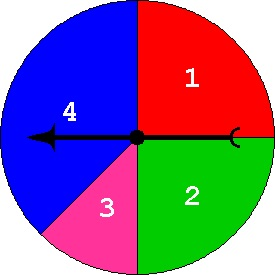
\includegraphics[scale=.5]{R1Spinner}
\end{multicols}

\item Consider the following carnival game.
The player pays $\$2$ to play the game, which
consists of spinning the spinner
shown in~(\ref{Spinner}). If the spinner stops in region~4
the player wins $\$4$. Otherwise the player wins nothing.
\begin{enumerate}
\item Calculate the expected proceeds for the player.
\item How can the game be made fair by modifying the
cost to play and the prize?
\end{enumerate}
\end{enumerate}
\end{document}
